% results.tex
\chapter{Results \& Discussion}

\section*{Genome Interaction Scaling}
In earlier treatments of the Hi-C data sets, the analysis of folding patterns by various groups \citep{imakaev2012} \citep{dixon2012}
the density of bound probes as a function of distance for the entire genome.  However, in our analysis, we remark that chromosomes
have heterogeneous scaling properties, as seen figure~\ref{fig:interactionScaling}.

\begin{figure}[h]
  \caption{Number of interactions as a function of distance.}\label{fig:interactionScaling}
\end{figure}

We find that the relative ordering of these curves are reproducible between replicates (Pearson=?).  This implies something.

Notably, the scaling ratios are unchanged by normalization, indicating that scaling may be a property of the underlying distribution
rather than an artifact of out data processing.  Indeed, this indicates that perhaps normalization should be performed, as is
done in HiCNorm \citep{hu2012} on a chromosome by chromosome basis, estimating different background distributions for each chromosome
rather than using a generalized fitting algorithm such as IPF\@.

\section*{Principal Components and Gene Expression}

We were curious whether a shift in the eigenvector for genomic regions could bring about a change in gene expression.  Using replicated
IMR90 and hESC gene expression experiments, we plotted the changes in gene expression against the compartment changes, but did not
find any correlation between changes in compartment character and gene expression levels ($\rho = -0.009$, $p$-value negligible.
See Figure~\ref{fig:expressionChangeByCompartment}.)

\begin{figure}[thp]
  \begin{minipage}{0.45\textwidth}%
    \centering
    \caption{Gene Expression Change by Compartment Change}\label{fig:expressionChangeByCompartmentChange}
    \includegraphics[width=\textwidth]{./figures/results/volcano.png}
  \end{minipage}

  \begin{minipage}{0.45\textwidth}
    \centering
    \caption{Compartmentalized Gene Expression}\label{fig:expressionChangeByCompartment}
    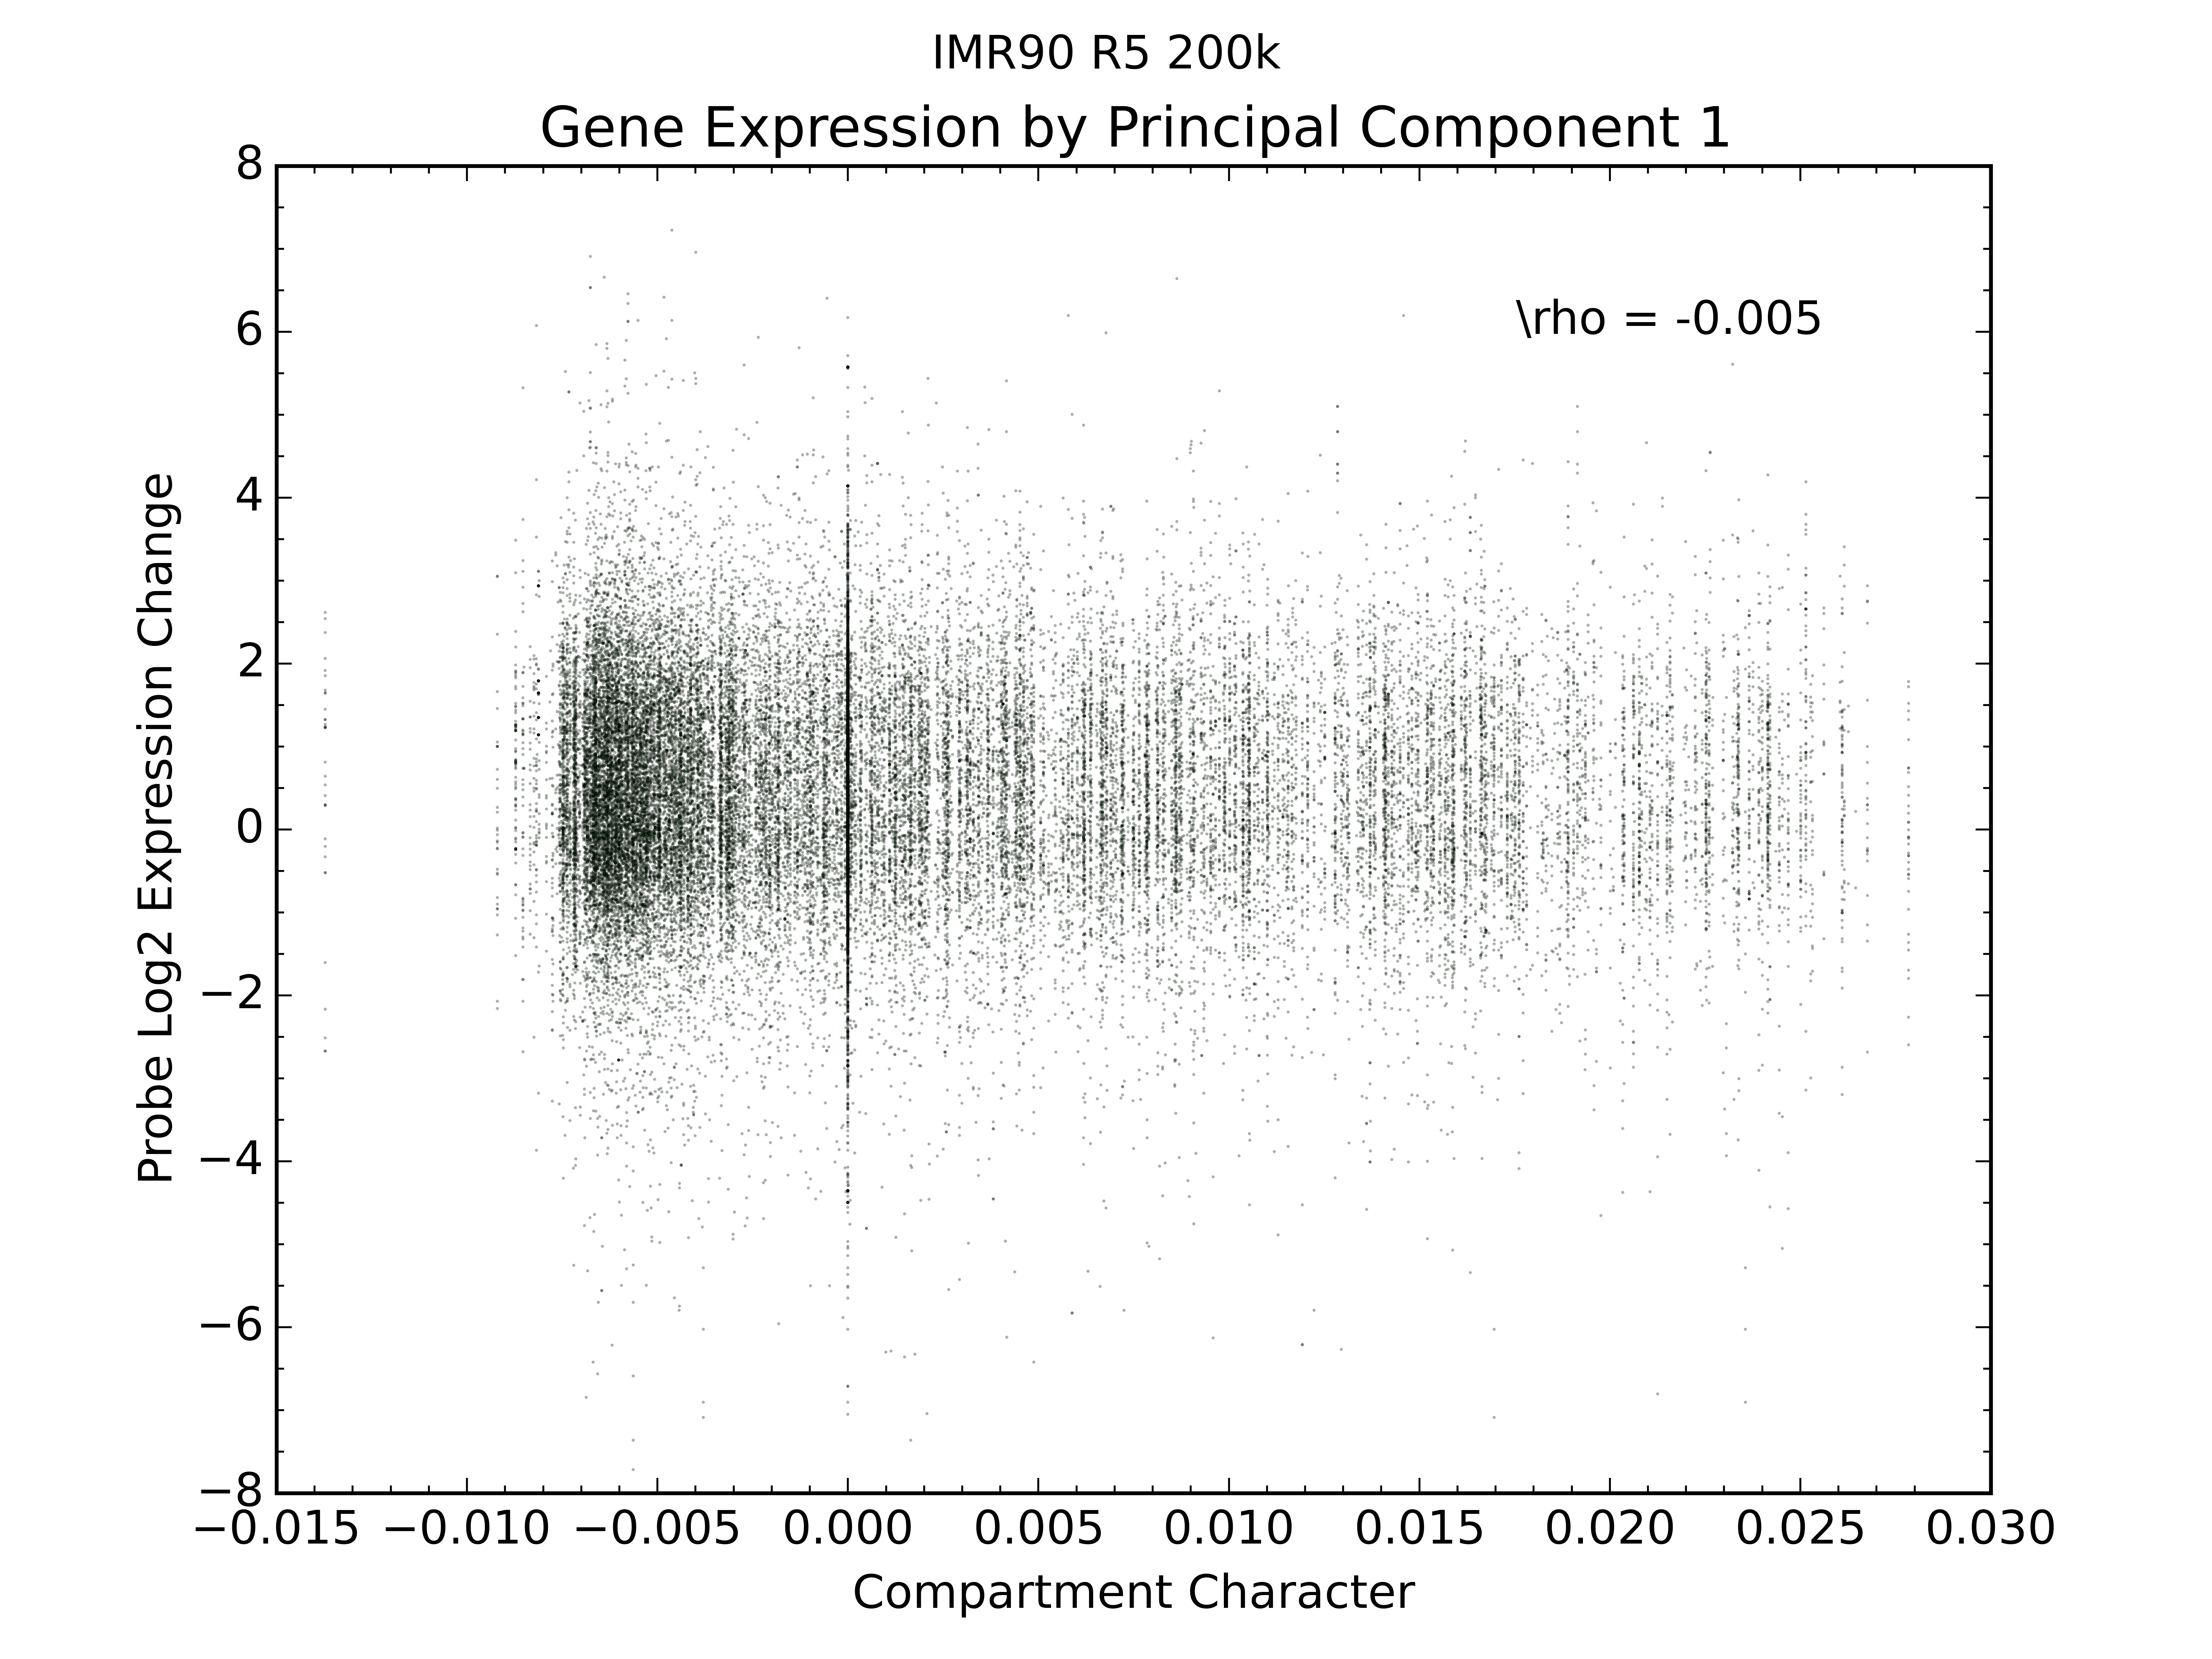
\includegraphics[width=\textwidth]{./figures/results/compartment_ir5_200k.png}
  \end{minipage}
\end{figure}

\section*{Eigenvector Partitioning}

The original Hi-C experiment revealed that the genome can be compartmentalized by \gls{PC} into two characteristic classes, arbitrarily 
labeled A and B.  Lieberman-Aiden and colleagues showed positive correlations between compartment identity, gene density, and chromatin
accessibility, concluding that compartment A consists of largely open chromatin, while compartment B is densely packed \citep{aiden2009}.
Interestingly, we did not observe any correlation between the eigenvector and gene expression data (via genome-wide mRNA expression,
Spearman's $\rho = -0.014$, p negligible; Supplementary Information~\ref{}).  Furthermore, shifts in compartment character did not correlate to 
changes in gene expression level (Spearman's $\rho = -0.01$, p negligible).  Given these results, it seems unlikely that cells regulate
gene expression at the compartment level.  Compartmentalization appears to be part of the larger nuclear architectural scheme, rather than
a dynamic regulatory mechanism.

Given the known differences between nuclear compartments, we investigated whether common fragile sites were clustered in a particular
compartment, conferring a level of fragility. 

\begin{figure}[thp]
  \centering
  \caption{Fragile Sites in Compartments}\label{fig:compartmentCfs}
  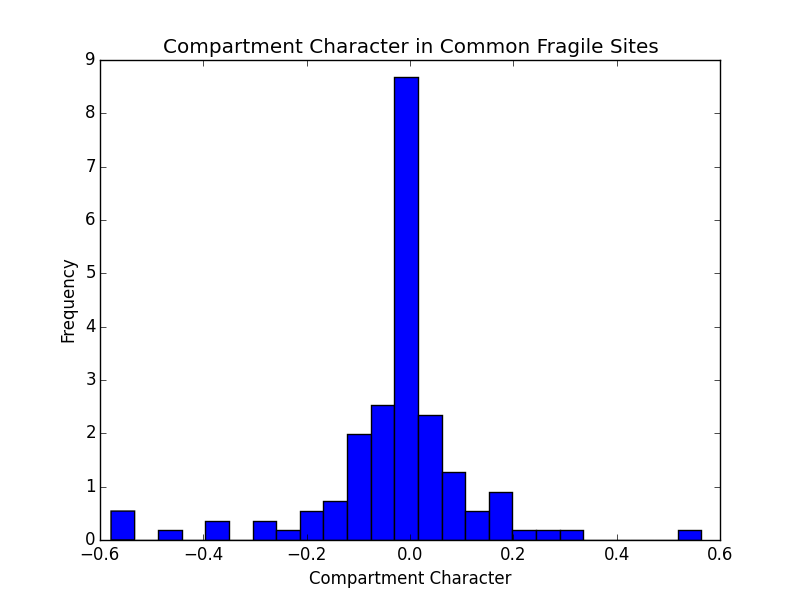
\includegraphics[width=\textwidth]{./figures/results/cfs.png}
\end{figure}



\section*{Directionality Indices}

If the nuclear architecture can be decomposed into layers as we have hypothesized, topological domains may exist at different
scales or resolutions within the nucleus.  We tested this hypothesis by calculating directionality indices at various window sizes
on a high resolution contact map.  Interestingly, we found that the minimum correlations between indices at a given window size increased
with higher resolution map ($\rho_{\min}(100kb) = 0.77, \rho_{\min}(1Mb) = 0.70$, Supplementary Information~\ref{sec:SuppDirectionality}).

\section*{Fragile Sites and Eigenvectors}

\section*{Domain Discovery}

The We dicovered a number of conserved domains between technical replicates of each cell line.  

\begin{figure}[thp]
  \caption{Number of Domains by Chromosome}
  \begin{minipage}{0.5\textwidth}%
    \centering
    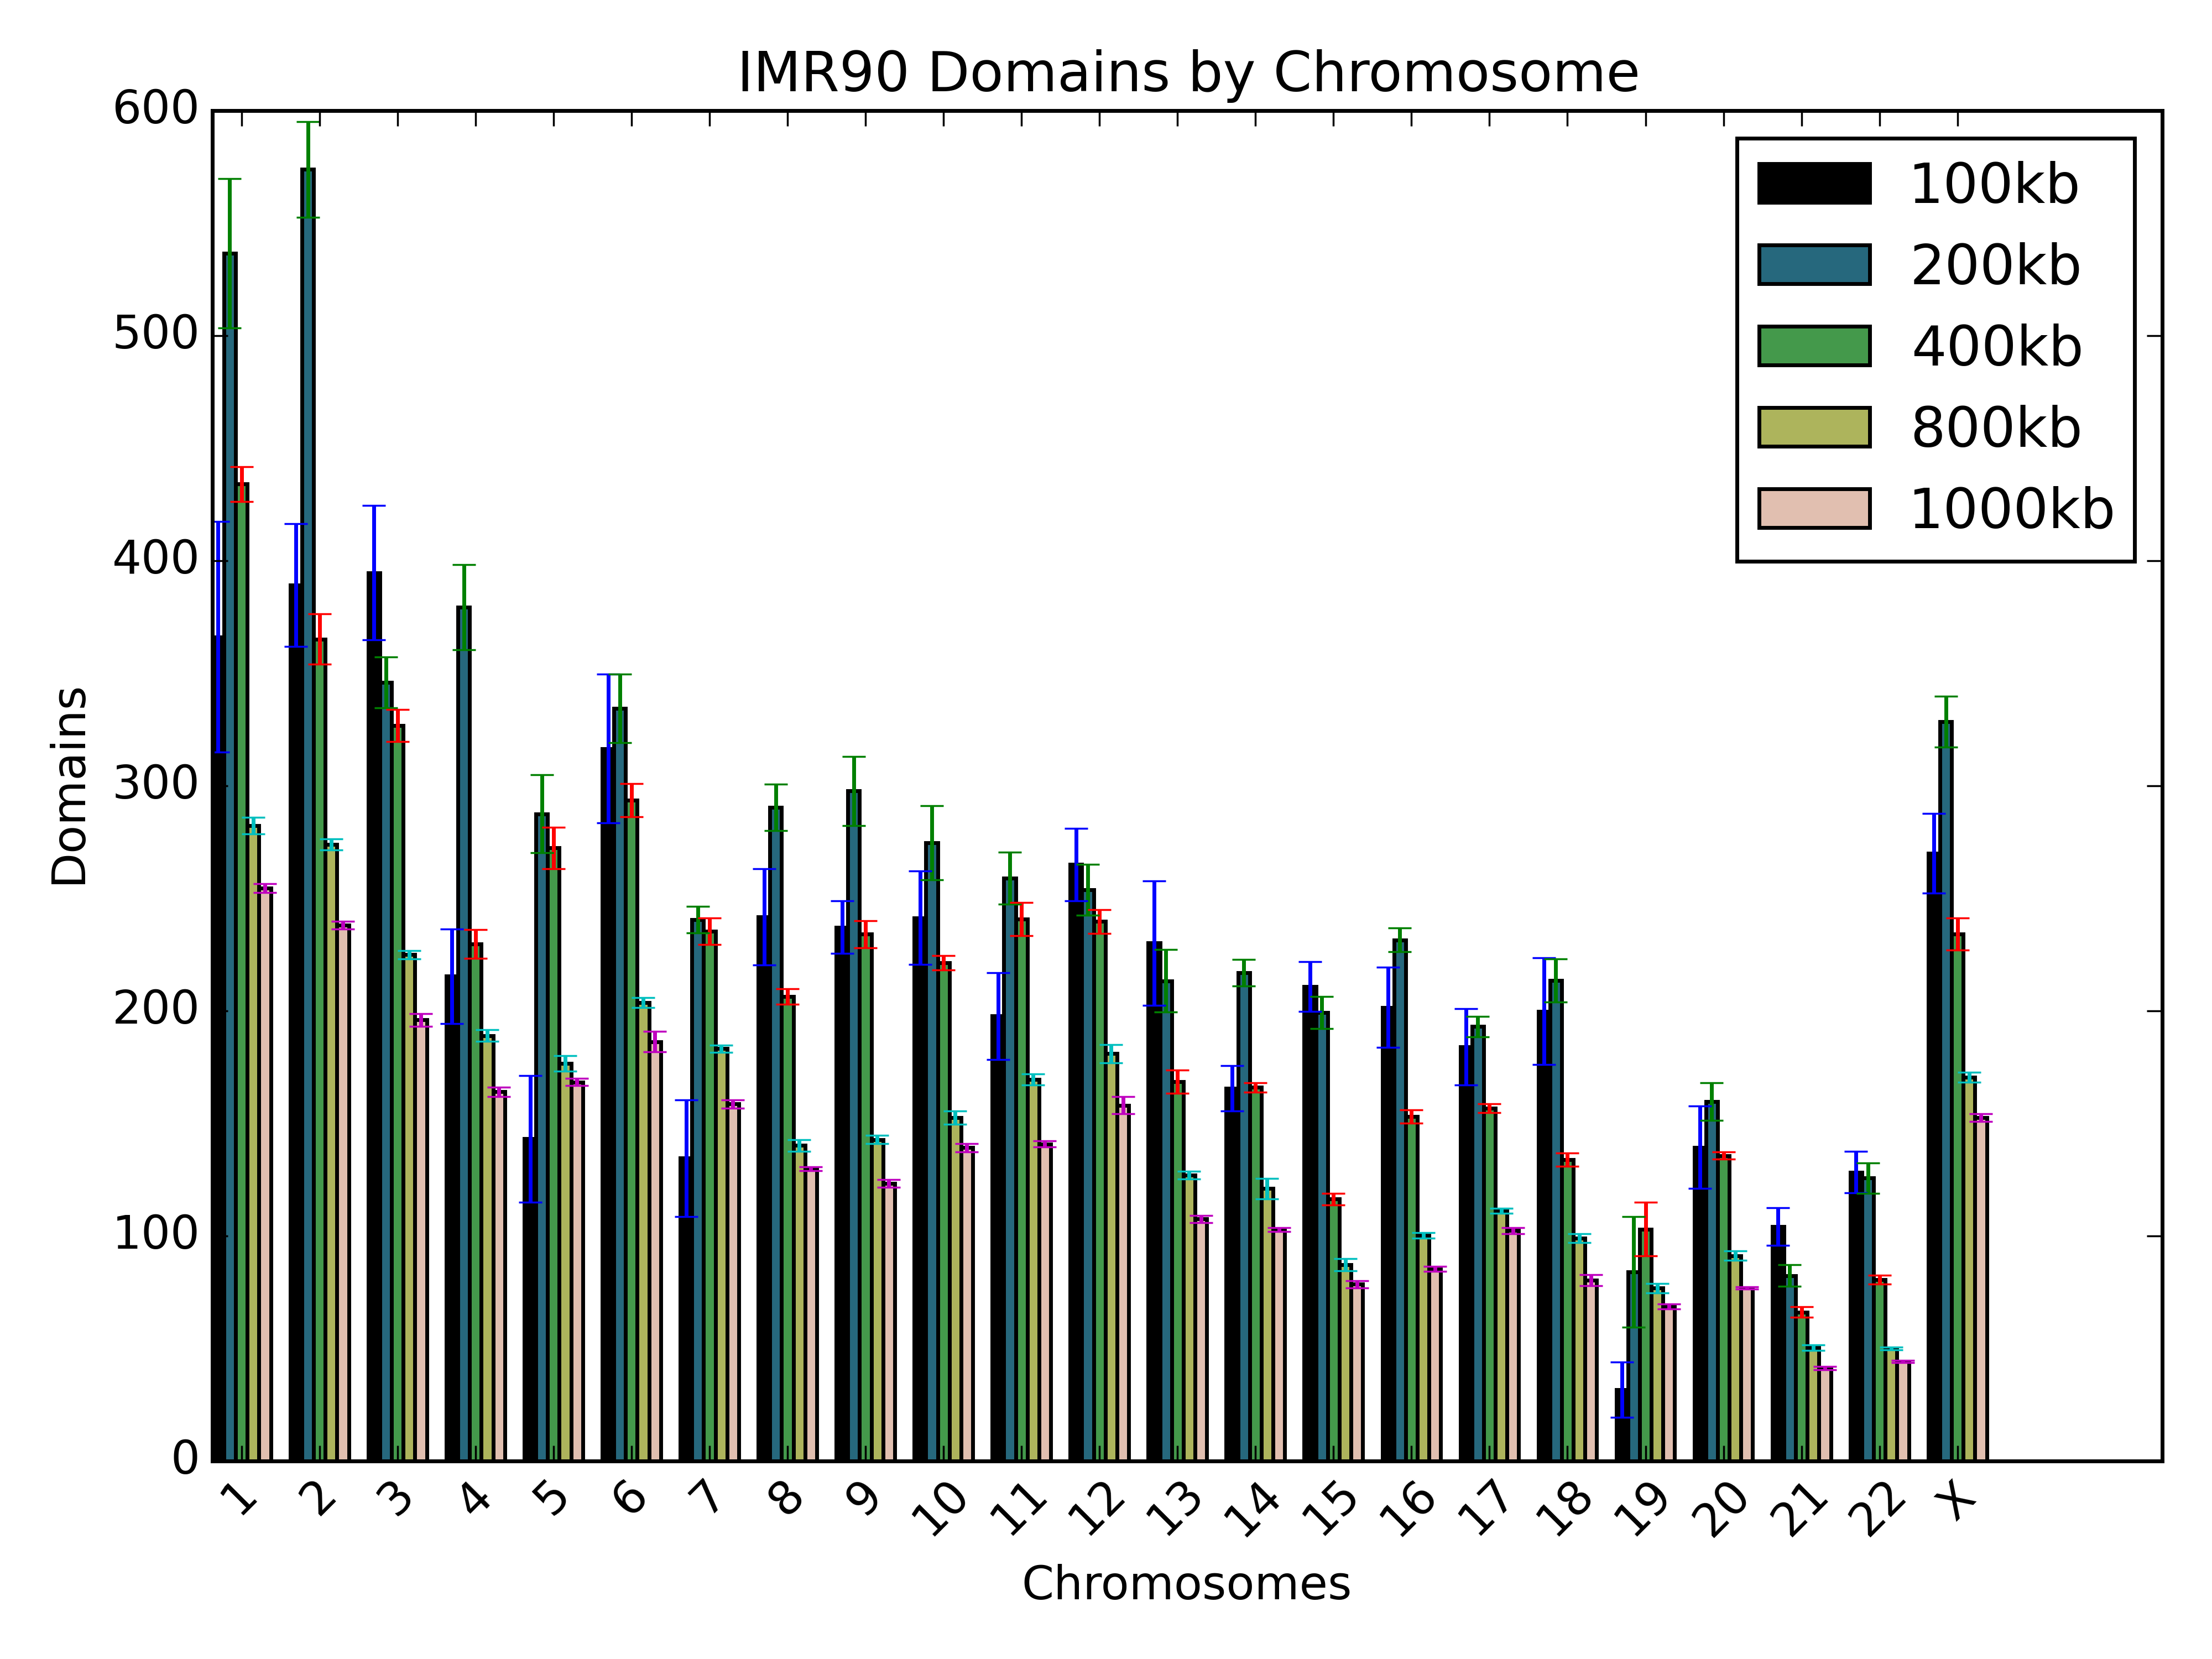
\includegraphics[width=\textwidth]{./figures/results/domain_imr90_bar.png}
  \end{minipage}

  \begin{minipage}{0.5\textwidth}
    \centering
    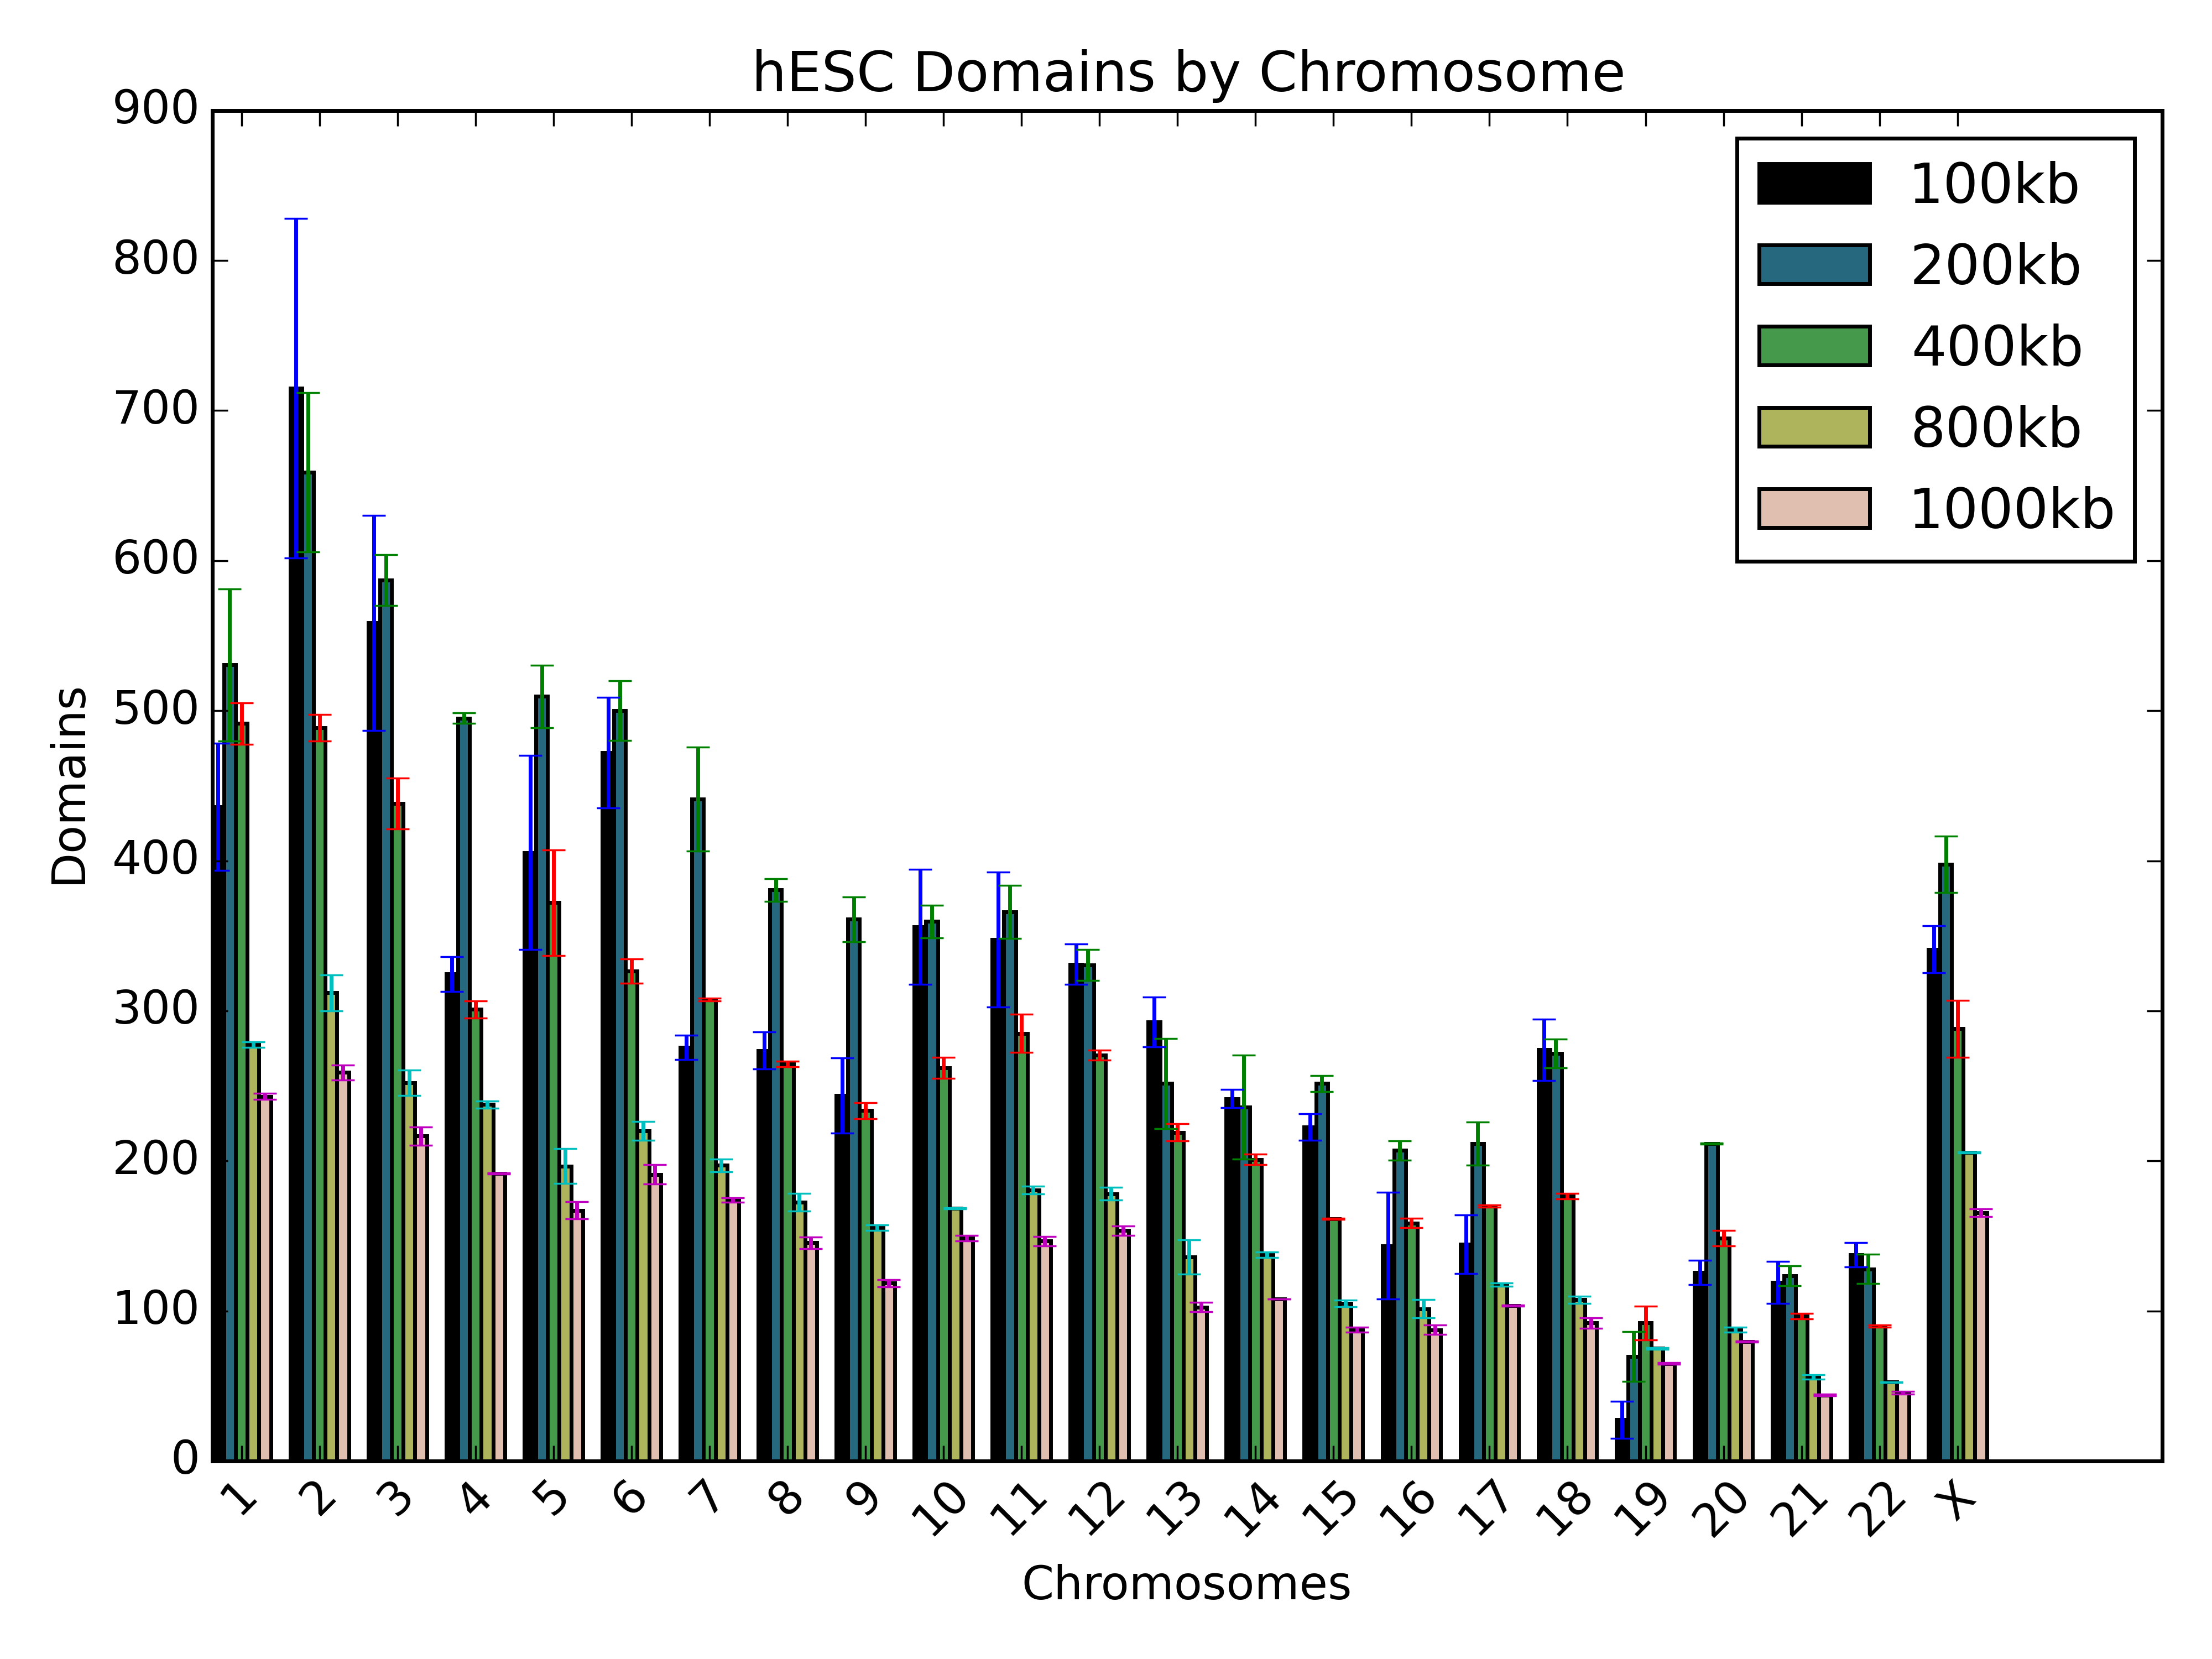
\includegraphics[width=\textwidth]{./figures/results/domain_hesc_bar.png}
  \end{minipage}
\end{figure}

\section*{Domain Boundary Proximity to Lesions}


